% SC3010 --- Chapter 3: Authentication (0->100 ground-up)
\chapter{Authentication: Passwords, MFA and Protocols}
\label{ch:auth}

\begin{quote}
\emph{``Authentication is proving you are who you claim to be.''} --- To a computer you are just bits on a wire; we must bind those bits to a human using something you know, have, or are.
\end{quote}

\noindent\fbox{\parbox{\dimexpr\linewidth-2\fboxsep-2\fboxrule}{%
\textbf{From zero: no crypto or security background assumed.} We start from everyday logins, build intuition with pictures, then formalise passwords, entropy, hashing, salting, multi-factor and biometrics, and finally dissect real protocols---challenge--response, Needham--Schroeder, and Kerberos. Every term is defined on first use.}}
\vspace{0.4em}

\section*{Learning Outcomes}
After this chapter you will be able to:
\begin{enumerate}[label=(L\arabic*)]
    \item define authentication vs.\ identification and quantify password strength via entropy;
    \item explain why passwords must be salted and hashed and evaluate storage schemes;
    \item compare MFA factors and quantify biometric trade-offs (FAR/FRR, EER);
    \item describe challenge--response and analyse Needham--Schroeder and its fix;
    \item trace Kerberos ticket exchange and reason about replay and freshness.
\end{enumerate}

% ============================================================
\section{Passwords: Intuition to Formal Storage}
\label{sec:passwords}
\paragraph{Intuition.} A password is a shared secret---like a clubhouse word. The server should recognise the word without storing it in plain text, because leaks happen. Instead it stores a one-way fingerprint.

\begin{definition}[Entropy and guessing]
If a password is drawn uniformly from $N$ possibilities, its entropy is $H=\log_2 N$ bits. A dictionary of $D$ candidates guesses correctly with probability $D/N= D\cdot 2^{-H}$.
\end{definition}
For 8 random lowercase letters, $N=26^8$, $H\approx 37.6$ bits. User-chosen words have far less: ``\texttt{p@ssw0rd}'' may be in a $10^6$-entry crack dictionary, so effective $H\approx 20$ bits.

\paragraph{Storing correctly.} Never store $pwd$. Store $h=H(salt\parallel pwd)$ with a unique random $salt$ per user and a slow hash (bcrypt/Argon2). Salt defeats rainbow tables; slowness defeats brute force.

\begin{figure}[h]\centering
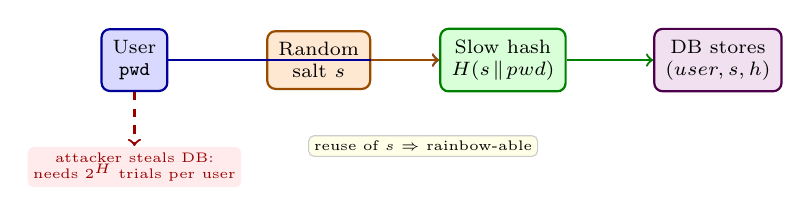
\begin{tikzpicture}[scale=0.78,every node/.style={font=\scriptsize},
  box/.style={draw,thick,rounded corners=3pt,align=center,inner sep=4pt}]
\node[box,fill=blue!15,draw=blue!60!black] (pwd) at (0,0) {User\\ \texttt{pwd}};
\node[box,fill=orange!18,draw=orange!60!black] (salt) at (3,0) {Random\\ salt $s$};
\node[box,fill=green!15,draw=green!50!black] (hash) at (6,0) {Slow hash\\ $H(s\!\parallel\!pwd)$};
\node[box,fill=violet!12,draw=violet!60!black] (db) at (9.5,0) {DB stores\\ $(user,s,h)$};
\draw[->,thick,blue!60!black] (pwd) -- (hash);
\draw[->,thick,orange!60!black] (salt) -- (hash);
\draw[->,thick,green!50!black] (hash) -- (db);
\draw[->,thick,red!60!black,dashed] (pwd) -- ++(0,-1.4) node[below,align=center,font=\tiny,fill=red!8,rounded corners=2pt,inner sep=2pt] {attacker steals DB:\\ needs $2^{H}$ trials per user};
\node[font=\tiny,fill=yellow!10,draw=gray!40,rounded corners=2pt,inner sep=2pt] at (4.7,-1.4) {reuse of $s$ $\Rightarrow$ rainbow-able};
\end{tikzpicture}
\caption{Password registration pipeline. Colour shows separation: blue secret, orange uniqueness, green one-wayness, violet stored verifier.}
\label{fig:pwd-pipeline}
\end{figure}

\begin{lstlisting}[language=Python,caption={Toy salted hashing. Production: use bcrypt/Argon2 with work factor.},label={lst:pwdhash}]
import hashlib, os
def register(pwd: str):
    salt = os.urandom(16)                      # 128-bit salt
    h = hashlib.sha256(salt + pwd.encode()).hexdigest()
    return salt.hex(), h                        # store (salt, h)

def verify(pwd: str, salt_hex: str, h: str) -> bool:
    salt = bytes.fromhex(salt_hex)
    return hashlib.sha256(salt + pwd.encode()).hexdigest() == h
# Attacker with DB still needs dictionary * slow-hash per salt
\end{lstlisting}

Offline guessing cost is $\approx D \times c_{\text{hash}}$; doubling hash time doubles attacker work. Online throttling and pepper ($HMAC_{k}$) add further defence.

\begin{example}[How fast is cracking?]
An 8-char random lowercase has $H=37.6$ bits $\approx 2\times10^{11}$ possibilities. At $10^9$ SHA-256/s (GPU) it falls in minutes; with bcrypt cost 12 ($\approx 0.3$s per hash) it needs $\approx 2000$ years. This is why ``fast hash $=$ broken storage'' and OWASP mandates memory-hard Argon2id.
\end{example}

\begin{definition}[Threat model for authentication]
\emph{Online guessing}: attacker tries logins against live server (rate-limited). \emph{Offline cracking}: attacker stole $(salt,h)$ and tests $H(s\parallel\text{guess})$ locally---only slowness and entropy help. \emph{Replay/eavesdrop}: attacker observes or replays messages; freshness (nonce/timestamp) is required.
\end{definition}

\paragraph{Identification vs.\ authentication vs.\ authorisation.} \emph{Identification} claims ``I am Alice'' (a username). \emph{Authentication} proves it (password/MFA). \emph{Authorisation} decides what Alice may do---the subject of Ch.~4. Confusing these collapses the reference monitor.

% ============================================================
\section{MFA and Biometrics}
\label{sec:mfa-bio}
Three factor classes: \emph{know} (password/PIN), \emph{have} (token/phone), \emph{are} (fingerprint/face). MFA requires $\ge 2$ distinct classes; two passwords is not MFA.

\begin{definition}[Biometric errors]
For threshold $t$, false accept rate $\text{FAR}(t)=P(\text{accept}\mid\text{impostor})$ and false reject $\text{FRR}(t)=P(\text{reject}\mid\text{genuine})$. The equal error rate $\text{EER}$ is where $\text{FAR}=\text{FRR}$.
\end{definition}
Tuning $t$ trades security (low FAR) against usability (low FRR). No biometric is secret---you leave fingerprints everywhere---so biometrics must be paired with liveness checks and revocable templates.

\begin{example}[Fingerprint vs.\ face]
Fingerprint EER $\approx 1\%$ at phone sensors; face under varied lighting may be $2$--$5\%$. A data centre ($10^4$ entries/day, 1 impostor/year) cannot tolerate FAR $=10^{-3}$ (10 false accepts/year) and pushes $t$ toward low FAR, accepting higher FRR and adding a fallback (PIN). Phones do the opposite: low FRR for convenience, compensating with short retry lockouts.
\end{example}

\paragraph{Why MFA can still fail.} SMS OTP is ``have'' but vulnerable to SIM-swap and SS7 interception---NIST 800-63B now discourages SMS. Push-based MFA suffers ``MFA fatigue'' where users approve spurious prompts. Strong MFA uses FIDO2/WebAuthn challenge--response with hardware keys: the ``have'' proves possession of a private key that never leaves the token.

\begin{figure}[h]\centering
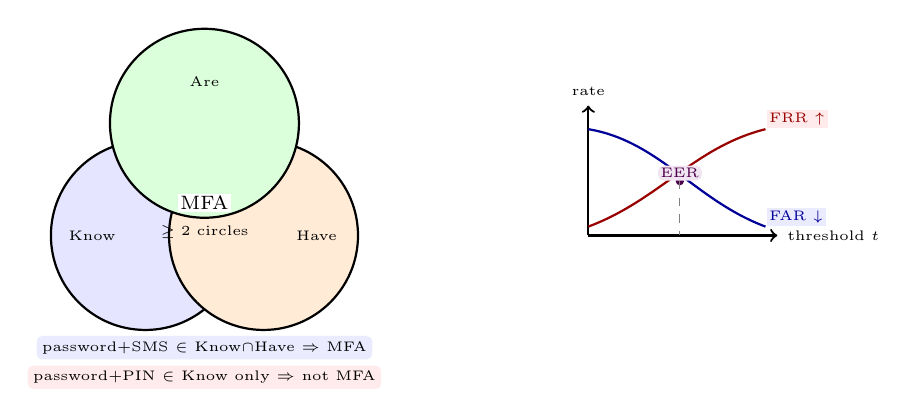
\begin{tikzpicture}[scale=0.75,every node/.style={font=\scriptsize}]
\draw[thick,fill=blue!10] (0,0) circle (1.6);
\draw[thick,fill=orange!16] (2.0,0) circle (1.6);
\draw[thick,fill=green!14] (1.0,1.9) circle (1.6);
\node[font=\tiny] at (-0.9,0) {Know};
\node[font=\tiny] at (2.9,0) {Have};
\node[font=\tiny] at (1.0,2.6) {Are};
\node[font=\scriptsize,fill=white,inner sep=1pt] at (1.0,0.55) {MFA};
\node[font=\tiny,align=center] at (1.0,0.05) {$\ge 2$ circles};
\node[font=\tiny,fill=blue!8,rounded corners=2pt,inner sep=2pt] at (1.0,-1.9) {password+SMS $\in$ Know$\cap$Have $\Rightarrow$ MFA};
\node[font=\tiny,fill=red!8,rounded corners=2pt,inner sep=2pt] at (1.0,-2.4) {password+PIN $\in$ Know only $\Rightarrow$ not MFA};
% FAR/FRR sketch
\begin{scope}[xshift=7.5cm]
\draw[->,thick] (0,0)--(3.2,0) node[right,font=\tiny] {threshold $t$};
\draw[->,thick] (0,0)--(0,2.2) node[above,font=\tiny] {rate};
\draw[thick,blue!60!black] (0,1.8) .. controls (1.2,1.6) and (1.8,0.6) .. (3.0,0.15) node[above right,font=\tiny,fill=blue!8,inner sep=1pt] {FAR $\downarrow$};
\draw[thick,red!60!black] (0,0.15) .. controls (1.2,0.6) and (1.8,1.5) .. (3.0,1.8) node[above right,font=\tiny,fill=red!8,inner sep=1pt] {FRR $\uparrow$};
\fill[violet!60!black] (1.55,0.92) circle (2pt) node[above,font=\tiny,fill=violet!10,rounded corners=2pt,inner sep=1pt] {EER};
\draw[dashed,gray] (1.55,0.92)--(1.55,0);
\end{scope}
\end{tikzpicture}
\caption{Left: MFA needs two distinct factor circles. Right: biometric threshold trades FAR against FRR; EER is the crossover.}
\label{fig:mfa-bio}
\end{figure}

% ============================================================
\section{Challenge--Response, Needham--Schroeder, Kerberos}
\label{sec:protocols}
\paragraph{Challenge--response.} The verifier sends a fresh nonce $N$; the claimant returns $F_K(N)$ (e.g.\ $HMAC_K(N)$). Freshness prevents replay. Without crypto, an eavesdropper replays.

\paragraph{Formal intuition.} An authentication protocol must guarantee \emph{aliveness} (peer recently participated), \emph{freshness} (message is not a replay), and \emph{binding} (key $K_{AB}$ is bound to $A$ and $B$, not an attacker). Needham--Schroeder aims to establish $K_{AB}$ with those three, but misses freshness for $B$.

\paragraph{Simple challenge--response (unilateral).}
\begin{lstlisting}[language=Python,caption={Toy challenge--response; real use: HMAC or signature.},label={lst:chal}]
import os, hmac, hashlib
K = os.urandom(16)                 # pre-shared key
def verifier_issue():  return os.urandom(16)         # nonce N
def prover_reply(N):   return hmac.new(K, N, hashlib.sha256).digest()
def verifier_check(N, tag): return hmac.compare_digest(prover_reply(N), tag)
# Reflection attack? Attacker reflects N back; include identities: HMAC(K, "B||N")
\end{lstlisting}

\paragraph{Needham--Schroeder symmetric (1978).} With key server $S$ sharing $K_{AS},K_{BS}$:
\begin{align}
1.\ & A\to S: A,B,N_A \nonumber\\
2.\ & S\to A: \{N_A,B,K_{AB},\{K_{AB},A\}_{K_{BS}}\}_{K_{AS}} \nonumber\\
3.\ & A\to B: \{K_{AB},A\}_{K_{BS}} \nonumber\\
4.\ & B\to A: \{N_B\}_{K_{AB}} \nonumber\\
5.\ & A\to B: \{N_B-1\}_{K_{AB}} \nonumber
\end{align}
Steps 4--5 authenticate $A$ to $B$ via nonce challenge. Flaw: if old $K_{AB}$ leaks, attacker replays message~3 and impersonates $A$ (no freshness for $B$). Denning--Sacco fix adds timestamps/extra nonce: $B$ checks recency.

\begin{theorem}[Needham--Schroeder flaw]
Without a freshness guarantee for $B$, compromise of a past session key $K_{AB}$ lets an attacker re-authenticate as $A$ indefinitely. Adding $T_B$ or requiring $B$ to consult $S$ restores authentication.
\end{theorem}

\begin{figure}[h]\centering
\begin{tikzpicture}[scale=0.78,every node/.style={font=\scriptsize},
  life/.style={thick,gray!60}, msg/.style={-{Stealth},thick,blue!60!black}]
\node[font=\small\bfseries] at (0,3.6) {A}; \node[font=\small\bfseries] at (4,3.6) {S (KDC)}; \node[font=\small\bfseries] at (8,3.6) {B};
\draw[life] (0,3.3)--(0,-2.2); \draw[life] (4,3.3)--(4,-2.2); \draw[life] (8,3.3)--(8,-2.2);
\draw[msg] (0,2.7)--(4,2.7) node[midway,above,font=\tiny,fill=blue!8,inner sep=1pt] {1.\ $A,B,N_A$};
\draw[msg,orange!70!black] (4,1.9)--(0,1.9) node[midway,above,font=\tiny,fill=orange!12,inner sep=1pt] {2.\ ticket$_{B}$ + $\{K_{AB}\}_{K_{AS}}$};
\draw[msg,green!50!black] (0,1.0)--(8,1.0) node[midway,above,font=\tiny,fill=green!12,inner sep=1pt] {3.\ \{K$_{AB}$,$A$\}$_{K_{BS}}$};
\draw[msg,violet!60!black] (8,0.15)--(0,0.15) node[midway,above,font=\tiny,fill=violet!10,inner sep=1pt] {4.\ $\{N_B\}_{K_{AB}}$};
\draw[msg,red!60!black] (0,-0.7)--(8,-0.7) node[midway,above,font=\tiny,fill=red!10,inner sep=1pt] {5.\ $\{N_B\!-\!1\}_{K_{AB}}$};
\node[font=\tiny,fill=red!8,draw=red!40,rounded corners=2pt,inner sep=2pt] at (8,-1.7) {replay ticket$_{B}$ if $K_{AB}$ leaked};
\end{tikzpicture}
\caption{Needham--Schroeder symmetric-key exchange. Messages 4--5 are the nonce challenge--response; lack of freshness in message~3 enables replay.}
\label{fig:needham}
\end{figure}

\paragraph{Kerberos (Needham--Schroeder fix deployed).} Realm with Authentication Server (AS) and Ticket-Granting Server (TGS). Timestamps replace nonces; tickets are \\
$\text{TGT}=\{A,TGS,K_{A\!-\!TGS},T_{exp}\}_{K_{TGS}}$, $\text{ST}=\{A,S,K_{A\!-\!S},T_{exp}\}_{K_S}$. Flow:
\begin{lstlisting}[language=Python,caption={Kerberos simplified flow (timestamps abbreviated).},label={lst:kerberos}]
# 1. Client -> AS : A, TGS, nonce
# 2. AS -> Client: {K_A_TGS, TGT}K_A   where TGT={A,K_A_TGS,exp}K_TGS
# 3. Client -> TGS: TGT, {A,time}K_A_TGS, S
# 4. TGS -> Client: {K_A_S, ST}K_A_TGS  where ST={A,K_A_S,exp}K_S
# 5. Client -> S : ST, {A,time}K_A_S
# 6. S -> Client: {time+1}K_A_S        # mutual auth
authenticator = HMAC(K_session, A + str(timestamp))
# S checks |clock - timestamp| < 5min and ST not expired
\end{lstlisting}
Kerberos adds real fix: short-lived tickets (typically 8--10\,h for TGT, minutes for ST), authenticators with timestamps, and a single sign-on. TGT lets Alice get STs without re-entering her password. Requires loosely synchronised clocks and careful replay cache. Mutual authentication comes from step~6: $S$ proves it knows $K_{A\!-\!S}$ by returning $\{time{+}1\}_{K_{A\!-\!S}}$.

\paragraph{Why timestamps and not more nonces?} Nonces need a round-trip and server-side state ($N$ pending). Timestamps are stateless: $S$ checks recency via $|\text{clock}-time|<\Delta$ plus a replay cache of recent authenticators. The price is clock sync (Kerberos needs NTP within $\approx 5$min) and the cache must be bounded to avoid DoS.

\begin{remark}[Public-key Needham--Schroeder and Lowe's fix]
The public-key variant ($A\to B:\{N_A,A\}_{K_B}$, $B\to A:\{N_A,N_B\}_{K_A}$, $A\to B:\{N_B\}_{K_B}$) falls to Lowe's interleaving attack: attacker $I$ posing as $A$ to $B$ reuses $B$'s challenge on $A$. Fix: include responder identity, $B\to A:\{N_A,N_B,B\}_{K_A}$. BAN logic (Burrows--Abadi--Needham) later formalised such reasoning.
\end{remark}

% ============================================================
\section{Exercises}
\label{sec:auth-exercises}
Each exercise ties intuition (why it matters) to a verifiable artefact (number, proof, trace).
\begin{enumerate}[label=E3.\arabic*, leftmargin=*, itemsep=0.6em]
    \item \textbf{Entropy maths.} A policy requires 10 characters from 94 printable ASCII uniformly. Compute entropy in bits and expected guesses for an attacker trying $10^9$ hashes/s with bcrypt cost $2^{12}$. Contrast with a 4-word Diceware phrase (7776-word list).
    \item \textbf{Salt and pepper.} Explain why per-user salt stops rainbow tables but not dictionary attacks, and what a server-side pepper $p$ (stored in HSM, used as $HMAC_p$) adds. What breaks if $p$ is checked into git?
    \item \textbf{Biometric tuning.} A face system has FAR$=10^{-3}$ and FRR$=0.05$ at threshold $t_0$. At $t_1$, FAR$=10^{-5}$, FRR$=0.20$. A building has 1000 staff entering twice daily and expects one impostor attempt per year. Compute expected false rejects and false accepts per year at each threshold. Which $t$ would you pick and why?
    \item \textbf{Needham--Schroeder replay.} Assume attacker learned $K_{AB}$ from a session last week and recorded $\{K_{AB},A\}_{K_{BS}}$. Walk through how they impersonate $A$ to $B$ step-by-step. Show how adding $\{B,N_B\}_{K_{BS}}$ or a timestamp in message~3 blocks the attack.
    \item \textbf{Kerberos clock skew.} Kerberos allows 5-minute clock skew. An attacker replays a captured ticket
    $\text{ST}$ with authenticator $\{A,time\}_{K_{A\!-\!S}}$ inside the window. How does the replay cache on $S$ prevent this, and what denial-of-service risk does a large cache create? Propose a nonce-based alternative and its cost.
\end{enumerate}

% ============================================================
\section*{Chapter Notes}
Morris--Thompson (1979) measured password guessability; Feldmeier--Karn (1990) and Boneh et al.\ catalogued Unix crypt evolution. Needham--Schroeder (1978) and Denning--Sacco (1981) framed freshness; Kerberos V5 (RFC~4120, Steiner--Neuman--Schiller) deployed the fix with tickets and timestamps---still the enterprise SSO backbone. For biometrics see Jain--Ross--Nandakumar and NIST 800-63B guidance on memorised secrets and MFA. FIDO2/WebAuthn (CTAP2) modernises challenge--response with public-key possession.

\paragraph{What to remember.} Good authentication is not ``clever passwords'' but architecture: slow salted hashes, MFA with independent factors, freshness in every protocol step, and short-lived tickets. When you next design a login, sketch the attacker with the DB, then check each message for replay.
% End of Chapter 3
